\documentclass[twocolumn,english,prb,showpacs,superscriptaddress]{revtex4-1}
\usepackage[colorlinks=true,urlcolor=blue,citecolor=blue,linkcolor=blue]{hyperref}
\usepackage[T1]{fontenc}
\usepackage[latin9]{inputenc}
\usepackage{amssymb}
\usepackage{graphicx}
\usepackage{amsmath,color}
\usepackage{mathrsfs}
\usepackage{float}
\usepackage{indentfirst}
\usepackage{babel}

% this is to be consistent with the newer PRB style
\usepackage[sort&compress]{natbib}
\setcitestyle{numbers,square}

\usepackage{color}

\newcommand{\bela}[1]{[\emph{\color{blue}{Bela: #1}}]}
\newcommand{\brayden}[1]{[\emph{\color{red}{Brayden: #1}}]}
\newcommand{\eqnref}[1]{Eq.~(\ref{#1})}

%\makeatletter

%%%%%%%%%%%%%%%%%%%%%%%%%%%%%%
%These may need modification
%\usepackage[section]{placeins}
\graphicspath{{../images/}{../diagrams/}{.}} %what folders to look for images in, via the command \includegraphics
\newcommand{\beq}{\begin{equation}}
\newcommand{\eeq}{\end{equation}}
\newcommand{\beqa}{\begin{eqnarray}}
\newcommand{\eeqa}{\end{eqnarray}}
\newcommand{\bi}{\begin{itemize}}
\newcommand{\ei}{\end{itemize}}
\newcommand{\ket} [1] {\vert #1 \rangle}
\newcommand{\bra} [1] {\langle #1 \vert}
\newcommand{\braket}[2]{\langle #1 | #2 \rangle}
\newcommand{\ev}[1]{\langle #1 \rangle}
\newcommand{\vbra}[1]{\left ( #1 \right |}
\newcommand{\vket}[1]{\left |#1 \right )}
\newcommand{\vbraket}[2]{\left ( #1 \middle |#2 \right )} 
\newcommand{\braopket}[3]{\left \langle #1 \middle |#2 \middle | #3 \right \rangle} 
\newcommand{\vbraopket}[3]{\left ( #1 \middle |#2 \middle | #3 \right )} 

%\newcommand<>{\highlighton}[1]{%
%  \alt#2{\structure{#1}}{{#1}}
%}

\newcommand{\icon}[1]{\pgfimage[height=1em]{#1}}

\usepackage{empheq}

\newlength\mytemplen
\newsavebox\mytempbox

\makeatletter
\newcommand\mybluebox{%
    \@ifnextchar[%]
       {\@mybluebox}%
       {\@mybluebox[0pt]}}

\def\@mybluebox[#1]{%
    \@ifnextchar[%]
       {\@@mybluebox[#1]}%
       {\@@mybluebox[#1][0pt]}}

\def\@@mybluebox[#1][#2]#3{
    \sbox\mytempbox{#3}%
    \mytemplen\ht\mytempbox
    \advance\mytemplen #1\relax
    \ht\mytempbox\mytemplen
    \mytemplen\dp\mytempbox
    \advance\mytemplen #2\relax
    \dp\mytempbox\mytemplen
    \fcolorbox{airlightblue}{white}{\hspace{1em}\usebox{\mytempbox}\hspace{1em}}}

\makeatother

\usepackage{wasysym}
\usepackage{amsfonts}
\usepackage{booktabs}
\usepackage{subfigure}
%%%%%%%%%%%%%%%%%%%%%%%%%%%%%%%

\begin{document}

\title{Not so featureless after all: \\ symmetry protected order in an interacting boson state}

\author{Brayden Ware}
\affiliation{Department of Physics, University of California, Santa Barbara, CA, 93106-6105, USA}

\author{Itamar Kimchi}
\affiliation{Department of Physics, University of California, Berkeley, CA 94720, USA}

\author{S. A. Parameswaran}
\affiliation{Department of Physics and Astronomy, University of California, Irvine, CA 92697, USA}

\author{Bela Bauer}
\affiliation{Station Q, Microsoft Research, Santa Barbara, CA 93106-6105, USA}

\begin{abstract}
While the Lieb-Schultz-Mattis theorem forbids the existence of fully 
symmetric quantum paramagnetic phases on lattices with fractional 
filling of particles per unit cell, such a phase is in principle 
allowed with certain fractional numbers of particles per site on 
non-Bravais lattices, including half-filling on the honeycomb lattice. 
It has been shown that a non-interacting Hamiltonian of spinless 
fermions or bosons cannot have such a symmetric insulating ground 
state, and an explicit construction using interactions is challenging. 
Recently, Kimchi et al. constructed a wavefunction for bosons at 
half-filling that does not break any symmetries and is not 
topologically ordered--and in this sense is a featureless insulator in 
the bulk. Here, however, we reveal that this wavefunction exhibits 
non-trivial structure at the edge. We apply recently developed 
techniques based on a tensor network representation of the 
wavefunction to demonstrate the presence of a gapless entanglement 
spectrum and a non-trivial action of combined charge-conservation and 
spatial symmetries on the edge. We will also discuss the possibility 
of finding a parent Hamiltonian and analyzing the existence of a 
symmetry-protected topological phase around this state.
\end{abstract}
\maketitle

%!TEX root = ../fbi.tex

\section{Introduction}


Featureless insulator problem description from   \onlinecite{parameswaran2013}
\bi 
\item Classical Mott insulators have integer site filling
\item LSM forbids featureless insulators at fractional unit cell 
filling. Site-filling can still be multiples of $1/n$
\item Extensions to LSM in \onlinecite{parameswaran2013-2} further 
forbid some site fractional site fillings for non-symmorphic lattices.
\ei 

In addition to finding featureless states, we also want to determine
 if different featureless states are in the same phase, i.e. whether 
 they can be connected without a phase transtion, but while preserving 
 the symmetry of the Hamiltonian H. Of particular interest are those 
 featureless states that cannot be connected adiabatically to a 
 product state without breaking the symmetry; these are called 
 symmetry protected topological (SPT) phases. Instead of local order 
 parameters, the distinguishing "features" of these phases appear at 
 phase boundaries, such as the edge of an open system, and in 
 entanglement properties of the bulk wavefunction.



 connecting path of Hamiltonians with featureless ground states everywhere along the path. Since the ground state degeneracy on a torus changes

SPT phases for a symmetry group G are featureless states 

The simplest example of a tensor network for a 1D system is a matrix 
product state; translationally-invariant matrix product states (MPS) 
are represented by a single rank 3 tensor $A_p^{ij}$ which specifies 
the wavefunction coefficients in a given basis local basis as a 
product of matrices $$\ket{\psi} = \sum\limits_{\{p_i\}} A_{p_1} 
A_{p_2} ... A_{p_N} \ket{p_0 p_1 ... p_N},$$ with one matrix for each 
site in the one-dimensional system.

PEPS are the generalization of MPS to two and higher dimensions, where 
each site in the system is represented by a rank $z+1$ tensor, where 
$z$ is the coordination number of the lattice, and wavefunction 
coefficients are similarly given by contracting over all virtual 
indices as shown in Figure \ref{fig:PEPS}.\cite{verstraete2004}
%!TEX root = ../fbi.tex

\section{Construction of the featureless boson insulator}
\label{sec:fbi}

\begin{figure}
	\centering
	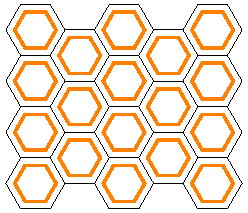
\includegraphics[width=0.6\columnwidth]{fbi3.pdf}
	\caption{Schematic representation of honeycomb FBI}
\end{figure}

In Ref.~\onlinecite{kimchi2013}, Kimchi et al gave an explicit
construction of a bosonic insulator
on the honeycomb lattice that is completely featureless in the bulk.
The state is succinctly described by the following wavefunction:
\begin{equation} \label{eq:def}
\ket{\psi} = \prod\limits_{\varhexagon} \sum\limits_{i \in
\varhexagon} b^{\dagger}_{i} \ket{0}.
\end{equation}
Here, $\varhexagon$ denotes the elementary hexagons of the honeycomb
lattice. We consider two closely related variants of the state, a
version of soft-core bosons where $b_i^\dagger$ creates a boson on
site $i$ and obeys the usual bosonic commutation relations, and a
hard-core version of the same state where $b_i^\dagger$ also creates a
boson but $(b_i^\dagger)^2=0$. In either case, the operator $\sum_{i
\in \varhexagon} b^{\dagger}_{i}$ creates exactly one boson per
hexagon; as there is one hexagon per unit cell of two sites of the
lattice, the state has one boson per unit cell, or half a boson per
site, thus allowing the existence of a featureless state.
In the case of soft-core bosons, the maximum number of bosons
per site is 3.

\bela{Summarize what was calculated in Ref.~\onlinecite{kimchi2013}.}

\subsection{PEPS representation}

In order to make the state~\eqnref{eq:def} more amenable to numerical
simulations, and in particular in order to be able to study its edge
properties, we now derive a representation as a projected entangled
pair states (PEPS). Importantly, this PEPS description will respect
all of the relevant symmetries of \eqnref{eq:def}.

\begin{figure}
	\centering
	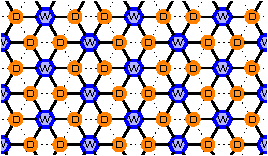
\includegraphics[width=0.8\columnwidth]{FBI_PEPS.pdf}
	\caption{\bela{Make labels math font. I think we might have to
	include physical indices in this figure, maybe very short/thin.}
	Intermediate tensor network for HFBI state. Here, the tensors labeled
	$D$ are located on the sites of the honeycomb lattice, while the
	tensors labeled $W$ are located on the centers of each hexagon.
	Dotted lines thus represent the physical lattice, while the solid
	lines indicate auxiliary bonds over which the tensor network is
	contracted. In this picture, we have suppressed the physical index
	for visual clarity.}
	\label{fig:FBI_PEPS}
\end{figure}

To obtain a PEPS construction, we first choose a local basis $\ket{n}$
of boson occupation numbers, i.e. $b^\dagger b \ket{n} = n \ket{n}$.
The PEPS will thus describe the coefficients of $\ket{\psi}$ in this
basis, $\langle n_1 \ldots n_L | \psi \rangle$. The PEPS
representation is most easily obtained in a two-step construction,
where we first construct the state shown in Fig.~\ref{fig:FBI_PEPS}.
Here, the tensor labeled $W=W^{n_1 \ldots n_6}$, which is placed in
the center of each hexagon, is a rank-6 tensor given by
\begin{equation}
W^{\{n_x\}}  = \left\{ \begin{array}{lr}
													1  : & \sum\limits_x n_x = 1 \\
													0  : & \text{else}
													\end{array} \right. .
\end{equation}
This tensor describes the coefficients of a so-called $W$-state in the
occupation number basis, i.e. $W^{\lbrace n_x\rbrace }= \langle n_1
\ldots n_6 | \sum_{i=1}^6 b_i^\dagger |0\rangle$. We note that this
tensor is symmetric under permutations of its indices.

On the sites of the physical lattice, we have placed a rank-4 tensor
denoted as $D$, shown in panel (a) of Fig.~\ref{fig:FBI_PEPS_2}, which
connects the $W$ tensors from three adjacent hexagons, and as fourth
index has a physical index $p$. For a state of soft-core bosons, where
$p=0,1,2,3$, this tensor is given by
\begin{equation} \label{eqn:D}
D^\mathrm{sc}_{p, i_0 i_1 i_2}  = \left\{ \begin{array}{ll}
													\sqrt{p!}  &: p =i_0+i_1+i_2  \\
													0  &:  \text{else}
													\end{array}
											\right. .
\end{equation}
We can also encode a state of hard-core bosons by replacing $D$ by
\begin{equation}
D^\mathrm{hc}_{p, i_0 i_1 i_2}  = \left\{ \begin{array}{ll}
													1  &: p = i_0+i_1+i_2 \le 1  \\
													0  &:  \text{else}
													\end{array}
											\right.
\end{equation}
Further variants of the state are described in
Appendix ~\ref{Appendix:Variants}.

This tensor network wavefunction manifestly respects all the
translational and point group symmetries of the honeycomb lattice,
since the tensors $W$ and $D$ are invariant under rotations of their
virtual indices in the plane. One can also check that the
wavefunction is $U(1)$ invariant with charge $1$ per plaquette.
\begin{figure}
	\centering
	\subfigure[D tensor]{%
		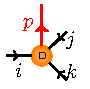
\includegraphics[width=0.18\columnwidth]{D_op.pdf}
		\label{fig:D}
	}
	\quad
	\subfigure[W-tensor and factored form]{%
		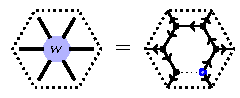
\includegraphics[width=0.5\columnwidth]{w_string.pdf}
		\label{fig:W}
	}
	\subfigure[PEPS tensor network for F.B.I. state]{%
		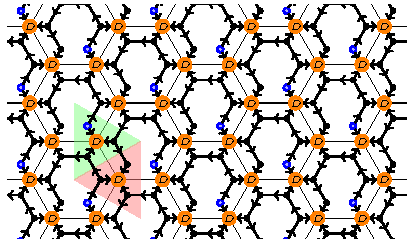
\includegraphics[width=0.8\columnwidth]{FBI_PEPS_2.pdf}
		\label{fig:FBI_PEPS_2A}
	}
\caption{\bela{I think the 1 in the center of the W MPS is confusing. Also, we should have shaded circles showing what the final PEPS tensor is.} Tensors used to put the F.B.I. tensor network in PEPS form. }
\label{fig:FBI_PEPS_2}
\end{figure}

In order to form a PEPS representation with all tensors located on the
vertices, we first factor the $W$-tensor into a matrix-product state
of six tensors as shown in panel (b) of Fig.~\ref{fig:FBI_PEPS_2}. We
choose a form of the MPS that breaks the rotational symmetry
of the W-state (which appears as translational symmetry of the MPS).
This allows us to obtain an MPS description with a small bond dimension
of $M=2$; a fully symmetric choice would require bond dimension 6.
Since these states are physically equivalent, we expect all
gauge-invariant quantities to be unaffected by this choice.
The decomposition is given by
\begin{equation}
W^{i_1 i_2 i_3 i_4 i_5 i_6} = \sum\limits_{\alpha_1 \ldots \alpha_5} V^{i_1}_{\alpha_1} W^{i_2}_{\alpha_1 \alpha_2}
%W^{i_3}_{\alpha_2 \alpha_3} W^{i_4}_{\alpha_3 \alpha_4}
\ldots
W^{i_5}_{\alpha_4 \alpha_5} X^{i_6}_{\alpha_5}
\end{equation}
where $V^{i_1}_{\alpha_1} = \delta_{i_1, \alpha_1}$, $X^{i_6}_{\alpha_5} = \delta_{i_6,\alpha_5+1}+\delta_{i_6,\alpha_5-1}$, and
\begin{equation*}
W_{i_0 i_1}^{j}  = \left\{ \begin{array}{ll}
													1  &:  i_0+j=i_1 \\
													0  &:  \text{else}
													\end{array}
											\right.,
\end{equation*}
where each index takes values in $\{0, 1\}$. Applying this to each
$W$-tensor yields the state as shown in panel (c) of
Fig.~\ref{fig:FBI_PEPS_2}. By contracting the three tensors in each
shaded region together, we obtain a PEPS in the regular form as shown
in Fig.~\ref{fig:PEPS}. The resulting PEPS has a bond dimension of
$M=2$ on the horizontal bonds, and a bond dimension of $M=4$ on all
other bonds. While it superficially breaks
the rotational symmetry of the lattice, it is an exact representation
of the FBI state and does not break any symmetries after contracting
the indices.

This decomposition respects the physical U(1) charge conservation
symmetry in that all tensors are separately
U(1)-invariant~\cite{bauer2011}. To make this manifest, we have
indicated in Fig.~\ref{fig:FBI_PEPS_2} arrows on each bond that show
the flow of charge.

\subsection{Representation on infinite cylinders}
For the calculations presented in this manuscript, we consider the
state $\ket{\psi}$ on a cylinder of infinite length, but finite
circumference $L$. In Fig.~\ref{fig:PEPS}, we have indicated the
choice of boundary conditions for the cylinder. For many practical
purposes, the PEPS on an infinite cylinder can be represented as an
infinite, translationally invariant matrix-product state of bond
dimension $2^L$.

\begin{figure}
	\centering
	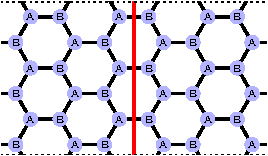
\includegraphics[width=\columnwidth]{Hex_PEPS.pdf}
	\caption{\bela{In this picture, we need to indicate the physical
	legs (maybe in a different color).} Pictoral representation of a
	PEPS on a honeycomb lattice. The tensors A and B are rank 4, with
	the physical leg at each site not shown for visual clarity. By
	gluing together the top and bottom edge of this picture, we get the
	"zig-zag" cylinder configuration used for most of the calculations
	in this paper. This cylinder is 3 unit cells wide, so we will call
	it the L=3 cylinder. In section \ref{sec:ES}, we will study the
	entanglement cut specified by the red line for various cylinder
	widths.}
	\label{fig:PEPS}
\end{figure}

%!TEX root = ../fbi.tex

\section{Correlation functions}

We use the the cylindrical geometry of Figure \ref{fig:PEPS} to compute correlation functions for this wavefunction. By looking at how the correlation length changes with cylinder width $L$, we conclude that indeed all correlations are exponentially decaying in the 2D limit of large $L$. 

\begin{itemize}
\item Show correlation bounds for soft-core and hard-core states, correlation function fits.

\begin{figure}[H]
	\centering
	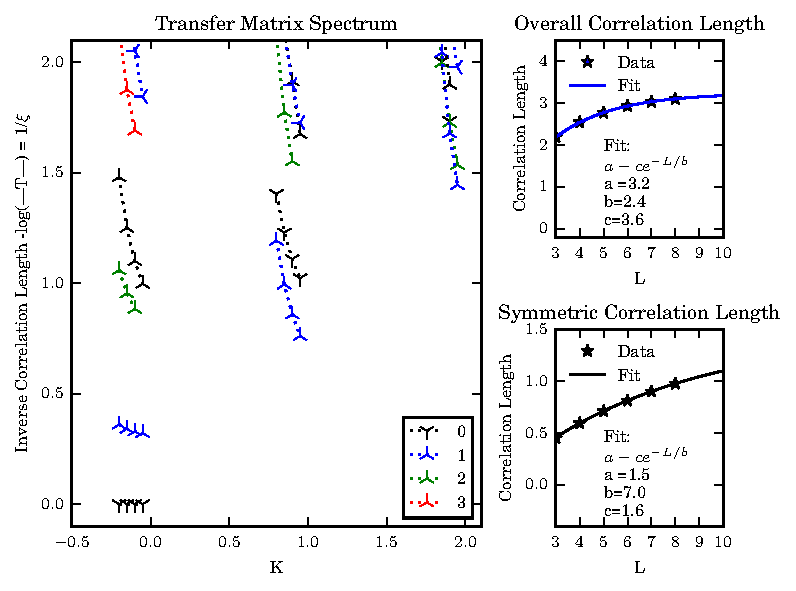
\includegraphics[width=\columnwidth]{TransferMatrixSpectrum_big.pdf}
	\caption{Placeholder for plots showing correlation bounds.}
	\label{fig:TMS}
\end{figure}

\item Emphasize that $\xi < L$ for the attainable system sizes $L$, so that we can have some trust in our results.
\item Show that correlations are isotropic.

\begin{figure}[H]
	\centering
	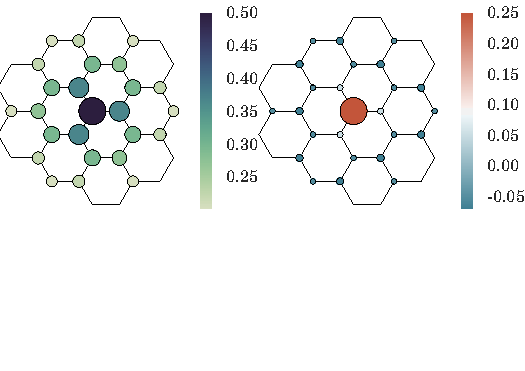
\includegraphics[width=0.6\columnwidth]{ShortDistanceCorrelations.pdf}
	\caption{Placeholder for 2D short distance correlation plot.}
	\label{fig:ShortCorr}
\end{figure}

\item Show that everything agrees with MC results, as far as those are available.
\end{itemize}



%!TEX root = ../fbi.tex

\section{Entanglement spectrum}
\label{sec:ES}

The quasi-1D cylinder geometry is also convenient for calculating the entanglement spectrum for 
entanglement cuts transverse to the cylinder. The procedure for computing the Schmidt decomposition is the 
same as for a MPS, and implies a canonical form for the quasi-1D MPS

$$
\ket{\psi} = \sum\limits_{\{p_i\}} \Gamma_{p_1} \Lambda \Gamma_{p_2} ... \Lambda \Gamma_{p_N} \ket{p_0 p_1 ... p_N}.
$$

The elements $\lambda_i$ of the diagonal matrix $\Lambda$ which appears in the canonical form,
are related to the non-zero eigenvalues $\rho_i$ of the reduced density matrix for the left or right half
of the system via $\rho_i = \lambda_i^2$.

The entanglement spectrum $\epsilon_i$  is defined via the equation $e^{-\epsilon_i} = \rho_i$. One says that the entanglement spectrum



Briefly discuss how the entanglement spectrum is calculated.\cite{cirac2011}

The entanglement spectrum shows a linear dispersion near momentum zero. Many points in the spectrum are 
doubly degenerate - those that are assigned a non-zero $U(1)$ charge.
	
\begin{figure}[H]
	\centering
	\includegraphics[width=\columnwidth]{{EntanglementSpectrum_L10.pdf}}
	\caption{Entanglement spectrum on a zig-zag edge L=10 cylinder}
	\label{fig:ESL10}
\end{figure}

On odd circumference cylinders, the entire entanglement spectrum is doubly degenerate.

\begin{figure}[H]
	\centering
	\includegraphics[width=\columnwidth]{{EntanglementSpectrum_L9.pdf}}
	\caption{Entanglement spectrum on a zig-zag edge L=9 cylinder}
	\label{fig:ESL9}
\end{figure}

The topological entanglement entropy is essentially zero.

\begin{figure}[hbctp]
	\centering
	\includegraphics[width=\columnwidth]{{TopologicalEntanglementEntropy.pdf}}
	\caption{The topological entanglement entropy $\gamma$ is consistent with 0.}
\end{figure}

The entanglement gap closes roughly as $1/L$. 

\begin{figure}[H]
	\centering
	\includegraphics[width=\columnwidth]{{EntanglementEnergyScaling.pdf}}
  \caption{Power law fits for the lowest five states above the ground state in Figure \ref{fig:ESL10}. The 
  $1/L$ scaling is a signature of a gapless (entanglement) Hamiltonian. Due to the small system size, 
  points at non-zero momentum still deviate significantly from $1/L$ scaling.}
\end{figure}

\newcommand{\uL}{\mathbf{L_0}}
\newcommand{\bL}{\mathbf{\bar{L}_0}}

\subsection{Identification of edge CFT}

Given the $U(1)$ symmetry of the state, the simplest possible conformal field theory we might expect to 
appear at the edge is that of a single free bosonic field. 

The free-boson CFT is created from the Lagrangian 
$$ \mathfrak{L} = \frac{g}{2}\int dt \int\limits_0^L dx ( \frac{1}{v^2}(\partial_t \phi)^2 - (\partial_x \phi)^2)$$
and with the compatified field identification
$$ \phi \equiv \phi + 2\pi R$$
and placed on the circle of circumference $L$ with periodic boundary conditions
$$ \phi(x) \equiv \phi(x+L).$$

After canonical quantization, it is found that the set of energy eigenstates consists of $U(1)$ Kac-Moody 
primaries $\ket{e, m}$, with integers $e, m$ labeling the $U(1)$ charge and the winding number of the 
bosonic field respectively, and level $n, \bar{n}$ descendant fields for each primary - such as  
$\mathbf{\bar{j}}_{-\bar{n}} \mathbf{j}_{-n} \ket{e, m}$ - for any nonnegative integers $n, \bar{n}$. The 
number of level $n, \bar{n}$ descendants of a given primary, all of which are degenerate, is $Z(n) 
Z(\bar{n})$, where $Z(n)$ is the number of partitions of the integer $n$.

The properties of the $U(1)$ Kac-Moody algebras constrain the form of energy and momentum eigenvalues - 
for the state $\mathbf{\bar{j}}_{-\bar{n}} \mathbf{j}_{-n} \ket{e, m}$, 

\begin{align*}
	\mathbf{P} =\frac{2\pi}{L}&(\uL-\bL) 
	&=& \frac{2\pi}{L}(em + n - \bar{n}) \\
	\mathbf{H} = \frac{2\pi}{L}&(\uL+\bL) 
	&=& \frac{2\pi}{L}(\frac{\kappa e^2}{2} + \frac{m^2}{2 \kappa} + \frac{n + \bar{n}}{2}) %\\
\end{align*}

By rescaling the energy and momentum, we find a system size independent pattern that can be matched to the 
low-energy, linearly dispersing part of the entanglement spectrum from Figures \ref{fig:ESL10} and 
\ref{fig:ESL9}. 

\begin{align*}
\mathbf{P} &\propto (em + n - \bar{n}) \\
\mathbf{H} &\propto e^2 + \frac{m^2}{\kappa^2} + \frac{1}{\kappa}(n + \bar{n})
\end{align*}

The label $m$ is 0 for all states in the linearly dispersing cone around $K=0$ - however, the primary 
states $\ket{e, m=\pm 1}$ can be found centered around momentum $K=\pi$, as seen in critical spin chains 
[reference]. The states with nonzero $e$ and zero $m$ are degenerate in energy and momentum with the same 
state with charge $-e$, but the $Z(n)Z(\bar{n})$ degeneracies predicted for descendant states are split by 
finite size effects.

The parameter $\kappa$ that appears - related to the coupling constant $g$ in the effective Lagrangian - 
is free. Quantum models that exhibit critical points that show the behavior of the free-boson CFT in fact 
have a whole line of critical points with varying values of $\kappa$, which can be tuned using a marginal 
operator in the theory.

\begin{figure}[H]
	\centering
	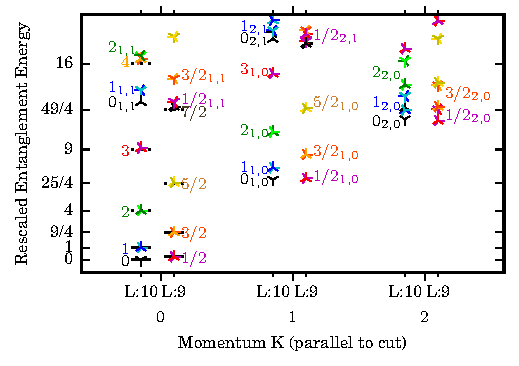
\includegraphics[width=\columnwidth]{EEIdentify.pdf}
	\caption{The identification of the primary states $\ket{\pm e, m=0}$ and the level $n, \bar{n}$ 
	descendants in the spectrum of the soft-core boson entanglement Hamiltonian. The states are labeled 
	$e_{n, \bar{n}}$. The zero and scale of the numerical spectrum are set by matching the lowest two 
	states. The energies and charges of the primaries with charges $2, 5/2, ... 4$ appear at the predicted 
	spots.  The best estimate for the Luttinger parameter from this spectrum is $\kappa \approx 1/6.4$, 
	taken from the energy of the $0_{1, 0}$ state. }
\end{figure}

We can also take the lowest-lying Schmidt state, interpret it as the ground state of a 1d Hamiltonian, and 
consider its entanglement.

\begin{figure}[H]
	\centering
	\includegraphics[width=\columnwidth]{{EdgeGS_EntanglementEntropy.pdf}}
	\caption{Entanglement entropy within the entanglement ground state of the soft-core boson state on $10$ 
	sites. For 	    comparison, the Cardy-Calabrese formula $S(x) = c/3 \log \sin( \pi x/L) + const.$ is 
	shown with $c=\frac{1}{2}, 1,$ and $2$, with the $const.$ fixed by matching the maximum of the 
	entanglement entropy data. $c=1$ is a good fit.}
	\label{fig:EdgeGS_EE}
\end{figure}



\subsection{Symmetry action on the edge}

\begin{figure}[H]
    \centering
    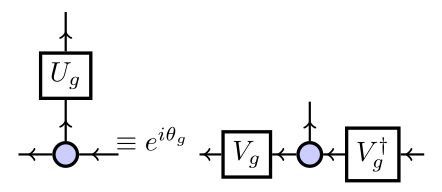
\includegraphics[width=0.6\columnwidth]{group_sym.png}
\end{figure}


\begin{figure}[H]
    \centering
    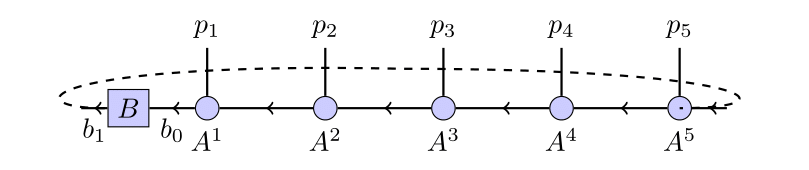
\includegraphics[width=\columnwidth]{mpsbc.png}
\end{figure}

\begin{tabular*}{\columnwidth}{@{\extracolsep{\stretch{1}}}*{5}{r}@{}}
\toprule
$\mathbf{G}$ & $\mathbf{U_g}$ & $\mathbf{\theta_g}$ & $\mathbf{V_g}$ &$\mathbf{V_g V^*_g}$ \\
\midrule
 $U(1)$ & & & & \\
 $\mathcal{\pi}$ & & & & \\
 $\mathcal{I}$ & & & & \\
 $\mathcal{\pi} \mathcal{I}$ & & & & \\
\bottomrule
\end{tabular*}

Since 
$$  
V_{\mathcal{\pi} \mathcal{I}} V_{\mathcal{\pi} \mathcal{I}}^* = -I \text{\quad or \quad } V_{\mathcal{\pi}} V_{\mathcal{I}} = - V_{\mathcal{I}} V_{\mathcal{\pi}},
$$ 

the representation is in the nontrivial class of 

$$
H^2(\mathbb{Z}_2 \times \mathbb{Z}_2^{\mathcal{I}}; U(1)) = \mathbb{Z}_2.
$$
%!TEX root = ../fbi.tex

\section{Quasi-local parent Hamiltonian and perturbations}

\label{sec:perturbations}
%!TEX root = ../fbi.tex

\section{Conclusion and Discussion}

\appendix

\section{Determining the edge action of the symmetry using MPS}
\label{Appendix:MPS}

We can use the formalism of MPS to assign an action
of the symmetry on the Schmidt states, and in particular for the charge and 
translation on-site symmetries the Schmidt states can be simultaneously assigned
charge and translation quantum numbers. This method of discovering the symmetry 
action will reproduce the action discussed in \ref{sec:ES} and quantum numbers used
in the spectra plots shown in Fig.~\ref{fig:ESL910}.
  
Let's discuss this formalism briefly. In addition,
we will discuss a generalization of this method that allows us to numerically
determine the symmetry action of inversion symmetry on the Schmidt states,
as in Section~\ref{sec:symmetry}. 
Both of these discussions follow Ref.~\onlinecite{pollmann2010}.

These discussions start by finding tensors $\Gamma, \Lambda$ representing the 
so-called canonical form of the MPS, as
originally detailed in \cite{perezgarcia2008}. This canonical form provides the Schmidt
decomposition at each site in the lattice.
\beq
\ket{\psi} = \sum\limits_{\{p_i\}} \ldots \Lambda \Gamma_{p_0} \Lambda \Gamma_{p_1} \Lambda \Gamma_{p_2} \Lambda \ldots \ket{... p_0 p_1 p_2 ...}.
\eeq
As a reminder, each physical leg represents all $2W$ physical sites on a cylinder slice,
and each virtual leg represents all virtual indices that connect cylinder slices.
The change of basis to canonical form generally mixes the Hilbert spaces from these
virtual legs, so the resulting basis won't be local around the circumference
of the cylinder.

Each on-site symmetry of the wavefunction $U_g = \otimes_i u^i_g$, with $U_g
\ket{\psi} = e^{i \Theta_g} \ket{\psi}$ is assigned an operator $V_g$ that
acts on the virtual leg of the MPS, that satisfies the equation
\begin{center}
\beq
\label{eq:onsitesym}
\eeq
\vskip-5em
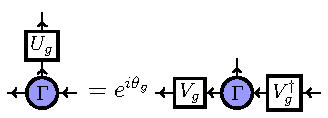
\includegraphics[width=0.6\columnwidth]{group_sym.pdf}.
\end{center}
This equation can be rewritten and solved as an eigenvector problem;
for an MPS with a nondegenerate largest transfer matrix eigenvalue,
this equation is guaranteed have a unique solution where the eigenvalue $e^{i \theta_g}$
is the largest eigenvalue of the eigenvector problem.

The solutions $V_g$ have two important properties: they are only defined up to a phase,
and they are guaranteed to commute with the diagonal matrix $\Lambda$ of Schmidt weights.  

Due to the first property, these operators are not guaranteed to form a linear
representation of the group of on-site symmetries, but in general could make
up a projective representation, satisfying
$$V_g V_h = e^{i \omega(g, h)} V_{gh}.$$ 
It is not always possible to absorb these phases into the definitions of the $V_g$.
The set of equivalent classes of phases $\omega(g, h)$ 
under redefinitions $V_g \to \alpha(g)V_g$ is called $H^2(G, U(1))$, the second group 
cohomology with $U(1)$ coefficients. 

For all the groups discussed in this paper, the group cohomology classes are labeled by
elements of a discrete abelian group - these discrete classes cannot be connected to each other
continuously. Physically, only a phase transition or breaking the symmetry allows one to connect
the different projective symmetry actions. 
Additionally, the classification of projective representations for the on-site symmetry group 
$U(1) \times \mathbb{Z}_W$ representing charge and translation around the cylinder is trivial. 
Thus, these edge symmetries can be taken to act linearly, 
and all Schmidt states can always be simultaneously assigned charge and momentum eigenvalues,
as in Figure~\ref{fig:ESL910}.

The second property guarantees that the $V_g$ only mixes exactly degenerate Schmidt states.
The action of $V_g$ must have the same phases $\omega(g, h)$ on each degenerate block of Schmidt 
states, so the projective representation can be nontrivial on any block only if every Schmidt 
state throughout the entire spectrum is degenerate. The degeneracy will be protected by the 
symmetry if and only if the $V_g$ form a nontrivial projective representation. Therefore
this 1D SPT analysis can only potentially give a nontrival answer for the odd $W$ states 
of the HFBI, where this exact degeneracy is seen throughout the spectrum. Nonetheless, we find 
there are no on-site symmetries of the wavefunction that can be used to explain the degenerate
entanglement spectrum of the odd $W$ HFBI states. Instead we must use an inversion symmetry. 

The MPS analysis of inversion symmetry works similarly. We will consider in general any symmetry  
$h$ of the wavefunction that squares to the identity and that can be written in the MPS as the 
product of an on-site symmetry action $U_h$ and a transpose of the site tensor.
This will include an inversion of the honeycomb lattice - equivalent to a 180 degree rotation 
about the center of any plaquette, which we label $\I = \I_y \I_x$, and the combination of
inversion with on-site symmetries. In addition, by blocking two site-tensors together, we
can write the reflection symmetry $\I_y$ in this form as well. In this scenario, the 
edge symmetry action satisfies
\begin{center}
\beq
\label{eq:onsitesym}
\eeq
\vskip-5em
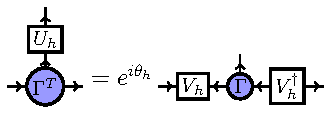
\includegraphics[width=0.6\columnwidth]{inv_sym.pdf}.
\end{center}
The map $V_{h}$ is also computed as a dominant eigenvector. 

For the HFBI, the symmetry group respected by the cylinder geometry is
$U(1) \times (\mathbb{Z}_W \rtimes \mathbb{Z}_2)
\times \mathbb{Z}_2^P \times \mathbb{Z}_2^T$, where the factors refer to charge
symmetry, translation around the cylinder, $\I_x$, $\I_y$, and $\tau$ respectively.
The $P$ and $T$ denote space-reversing and time-reversing symmetries, and signify the 
antiunitary action on the Schmidt states. 
%Compute the cohomology class of 
%$H^2(U(1) \times (\mathbb{Z}_W \rtimes \mathbb{Z}_2)
%\times \mathbb{Z}_2^P \times \mathbb{Z}_2^T ; U(1)) ?$
Many of the non-trivial projective
representations of such a complicated group will remain projective when the symmetry is
restricted to a subgroup - in this case, the full symmetry is not needed to protect the 
entanglement degeneracy. As shown in Table~\ref{table:sym}, the projective representation 
corresponding to the HFBI state can indeed be protected by any one of a number of subgroups 
of the full symmetry group, all involving inversions and charge parity.

The symmetry actions - both on-site and inversion symmetries -
are computed in the Schmidt basis, but can be transformed
into the basis $\vket{\{\sigma_i\}}$ determined by the virtual legs of the PEPS in
Figure~\ref{fig:FBI_PEPS_2}. 
In this case, the symmetry action $V_{\I_y}$ is precisely
a particle-hole symmetry in the local PEPS basis, with coefficients
$$
V_{\I_y}\vket{\sigma_1, \ldots, \sigma_{W}} = \vket{1-\sigma_1, \ldots, 1-\sigma_{W}}, 
$$
since a state where the $i^{th}$ hexagon contributes $\sigma_i$ bosons on the right is paired with
a state where the $i^{th}$ hexagon contributes $1-\sigma_i$ on the left.
Thus 
$$
V_{\I_y} = \prod\limits_i \sigma_i^x K,
$$
where K is complex conjugation in the local PEPS basis, and $\sigma_i^x$ is the Pauli
operator acting on the $i^{th}$ site of the local PEPS basis.

Charge symmetry acts locally as well:
$$
e^{i \theta \mathcal{Q}}\vket{\sigma_1, \ldots, \sigma_{W}} = e^{i \theta \sum(\sigma_i-1/2)}\vket{\sigma_1, \ldots, \sigma_{W}}.
$$
In particular, charge parity $V_{\varPi} = e^{i \theta \mathcal{Q}}$ can be written as
$$V_{\varPi} = e^{i \pi \sum(\sigma_i - 1/2)} = \prod\limits_i \sigma_i^z.$$

The combined action of charge parity and reflection across the cut takes the form 
$$
V_{\varPi \I_y} = \prod\limits_i \left(i \sigma_i^y \right) K,
$$
which is precisely the form that time-reversal acting on an ordinary spin-$\frac12$ chain takes.
When the circumference of the cylinder $W$ is odd, we see that
$$V_{\varPi \I_y}V_{\varPi \I_y}^{*} = -I.$$ 
The degeneracy of the entanglement spectrum can be seen as an application of Kramer's theorem.
Formally, this property is said to characterize the nontrivial projective representation
$$
H^2(\mathbb{Z}_2^P; U(1)) = \mathbb{Z}_2,
$$
and remains true while $\varPi \I_y$ is a symmetry and no phase transitions have occurred.

Time reversal symmetry acts as complex conjugation in the local PEPS basis $V_{\tau}=K$.
Translation and $\I_x$ act as permutations of the local PEPS basis:
\begin{equation*}
\begin{split}
V_{T}\vket{\sigma_1, \ldots, \sigma_{W}} &= \vket{\sigma_2, \ldots, \sigma_{W}, \sigma_{1}} \\
V_{\I_x}\vket{\sigma_1, \ldots, \sigma_{W}} &= \vket{\sigma_W, \ldots, \sigma_{1}}.
\end{split}
\end{equation*}
These symmetries can be combined with $V_{\varPi \I_y}$ to create the additional topological 
invariants shown in Table~\ref{table:sym}. A non-trivial projective 
representation in $$H^2(\mathbb{Z}_2 \times \mathbb{Z}_2; U(1)) = \mathbb{Z}_2$$
is created whenever two unitary symmetries that commute in the bulk satisfy 
$$V_{g_1} V_{g_2} V_{g_1}^{-1} V_{g_2}^{-1} = -I.$$
Each new invariant is related to a new set of pertubations that can't break the entanglement 
degeneracy. 

\section{Local Hamiltonian for the Edge free boson CFT}
\label{Appendix:LocalEdge}

B

\section{Mode expansion and symmetry action of free-boson CFT}
\label{Appendix:CFT}
How do the symmetry protecting operations act on the CFT states
$\ket{e, m, \{n_i\}, \{\bar{n}_i\}}$?

From that, infer how they act on the free boson fields $\phi$ and $\theta$.

Which perturbations to the CFT gap it out completely or spontaneously break the symmetry?

Are those pertubations forbidden by the implementation of symmetry on the edge.

\section{Variants on the HFBI wavefunction}
\subsection{Tuning soft-core bosons to hard-core}
In Equations~\eqref{eqn:Dsc} and \eqref{eqn:Dhc}, the tensor $D$ can be replaced by a more general form 
\begin{equation} \label{eqn:Dgen}
D_{p, i_0 i_1 i_2}  = \left\{ \begin{array}{ll}
													d_p  &: p =i_0+i_1+i_2  \\
													0  &:  \text{else}
													\end{array}
											\right. ,
\end{equation}
which the coefficients $d_p = 1,\, 1,\, \sqrt{2},\,\sqrt{6}$ for $p = 0,\, 1,\, 2,\, 3$ in the soft-core state and $d_p = 1,\, 1,\, 0,\, 0$ for $p = 0,\, 1,\, 2,\, 3$ in the hard-core state. We can continously tune the coefficients $d_2$ and $d_3$ from the soft-core to the hard-core values.
Upon doing so, we find that the transfer matrix spectrum remains gapped, with the correlation length monotonically increasing from the soft-core state to the hard-core state. 
Furthermore, the low energy parts of the entanglement spectrum do not change significantly through this tuning.
Therefore we expect that the hard-core and soft-core phases can be adiabatically connected with a 
path of local Hamiltonians, and all SPT results that apply to one state apply to the other. By choosing appropriate values of $d_2$ and $d_3$, we can also make replace the vacuum $\ket{0}$ in
Equation~\eqref{eq:def} with a constant background of $N$ filled bosons $\ket{N}$, or even make
states of spins $S$ where Equation~\eqref{eq:def} becomes
\begin{equation} \label{eq:spindef}
\ket{\psi} = \prod\limits_{\varhexagon} \left( \sum\limits_{i \in \varhexagon} S^{+}_{i} \right) \ket{S_z = m}.
\end{equation}

\subsection{Inversion Protected Phase}
Additionally, the tensor $W$ in Equation~\eqref{eq:W} can be replaced by the more general form
\begin{equation} \label{eq:Wgen}
W^{n_1 \ldots n_6}  = \left\{ \begin{array}{lr}
													p_x  : & n_x=1,\, n_y = 0
													\; \forall \; y \neq x \\
													0  : & \text{else}
													\end{array} \right.,
\end{equation}
which corresponds to modifying Equation~\eqref{eq:def} to 
\begin{equation} \label{eq:pdef}
\ket{\psi_{\ell}} = \prod\limits_{\varhexagon} \left( \sum\limits_{i \in \varhexagon} p_i b^{\dagger}_{i} \right) \ket{0}.
\end{equation}

This does not in general preserve the rotational symmetry of the state, but it does if the 
coefficients $p_0, \ldots p_5$ are in an angular momentum mode $$p_x = e^{i x \ell}$$ where
$\ell \in \{0, 2\pi/6, \ldots 5\pi/6 \}$. These 6 discrete solutions can't be continously tuned to one another while preserving all the lattice symmetries.

The state $\ket{\psi_{\ell=\pi}}$ can be shown to be related to state $\ket{\psi_{\ell=0}}$ discussed in the main text by a on-site unitary operator $U(\pi)$, 
where 
\begin{equation} \label{eq:Uphi}
U(\varphi) = \prod\limits_{j \in B} e^{i \varphi \hat{Q}_j}.
\end{equation}
Due to this relation, $\ket{\psi_{\ell=\pi}}$ and $\ket{\psi_{\ell=0}}$ have identical correlation lengths and entanglement spectra. 
However, the protecting symmetries from Table~\ref{table:sym} are mapped using conjugation
by $U(\pi)$ into a new set of protecting symmetries, shown in Table~\ref{table:pisym}. 

\begin{table}
\begin{tabular*}{\columnwidth}{@{\extracolsep{\stretch{1}}}*{4}{r}@{}}
\toprule
Group & Generators & Invariant & $i$  \\
\midrule
$\mathbb{Z}_2^P$ & $\{\I \}$ 
& $V_{\I} V_{\I}^* = -I$ &$-$ \\
$\mathbb{Z}_2^P$ & $\{\I_y \}$ 
&$V_{\I_y} V_{\I_y}^* = -I$ &$-$ \\ \hline
$\mathbb{Z}_2 \times \mathbb{Z}_2^{PT}$& $\{\varPi, \tau \varPi \I\}$ 
&$V_{\varPi} V_{\tau \varPi \I} V_{\varPi}^{-1} V_{\tau \varPi \I}^{-1} = -I$ &$+$ \\
$\mathbb{Z}_2 \times \mathbb{Z}_2^{PT}$& $\{\varPi, \tau \varPi \I_y\}$
&$V_{\varPi} V_{\tau \varPi \I_y} V_{\varPi}^{-1} V_{\tau \varPi \I_y}^{-1} = -I$ &$+$ \\
$\mathbb{Z}_2 \times \mathbb{Z}_2^{PT}$& $\{\varPi \I_x, \tau \varPi \I\}$
&$V_{\varPi \I_x} V_{\tau \varPi \I} V_{\varPi \I_x}^{-1} V_{\tau \varPi \I}^{-1} = -I$&$+$ \\
$\mathbb{Z}_2 \times \mathbb{Z}_2^{PT}$& $\{\varPi \I_x, \tau \varPi \I_y\}$
&$V_{\varPi \I_x} V_{\tau \varPi \I_y} V_{\varPi \I_x}^{-1} V_{\tau \varPi \I_y}^{-1} = -I$ &$+$\\
\bottomrule
\end{tabular*}
\caption{Summary of symmetry protecting invariants found for the $\ket{\psi_{\ell=\pi}}$ state. 
The degenerate entanglement spectrum cannot be split unless all 6 of the  minimal protecting symmetry groups are broken. }
\label{table:pisym}
\end{table}

Notably,
since
$$
U(\pi) \varPi \I U(\pi)^{\dagger} = \I, 
$$
this state has doubly degenerate entanglement spectra on odd cylinder sizes protected by lattice inversion symmetry alone.

A similar mapping for 1-D inversion protected states is discussed in Appendix A of Ref.~\onlinecite{pollmann2010}. As discussed \brayden{somewhere}, the state $\ket{\psi_{\ell=0}}$
on the $W=1$ cylinder is adiabatically connected to the 1-D Haldane insulator state discussed in
Ref.~\onlinecite{pollmann2010}. The new $\ket{\psi_{\ell=\pi}}$ state on the $W=1$ cylinder is instead adiabatically connected to the 1-D AKLT state. 

\label{Appendix:Variants}

\acknowledgements

\bibliography{fbi}

\end{document}
